\begin{figure}[H]
	\center
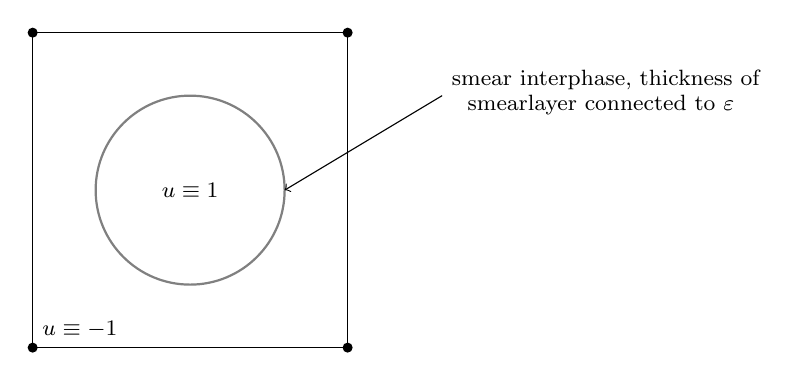
\begin{tikzpicture}[scale=4]
		
		\def \xone{0};
		\def \yone{0};		
		% first rectangle
		\coordinate (A) at (\xone,\yone);
		
        \draw (A) -- ++(0,1) -- ++(1,0)-- ++(0,-1) --cycle;
        \draw[thick,gray] (A) ++(0.5,0.5) circle (0.3cm);
        \filldraw (A)         circle (0.4pt);
        \filldraw (A) ++(1,0) circle (0.4pt);
        \filldraw (A) ++(0,1) circle (0.4pt);
        \filldraw (A) ++(1,1) circle (0.4pt);
        \fill[black,font=\footnotesize] (A)         node[above right] {$u \equiv -1$}
                                        (A) ++(0.5,0.5) node {$u \equiv 1$}
                                        (A) ++(1.3,0.85) node[right] {smear interphase, thickness of }
                                         (A) ++(1.35,0.77) node[right] {smearlayer connected to $\varepsilon$};
        \draw[-to] (A) ++(1.3,0.8) -- ++(-0.5,-0.3);
        
\end{tikzpicture}

\caption{Visualisation of motivation for pde}
\label{ch_mult_hahn_hilliard}
\end{figure}